Eventbrite, jako platforma internetowa, pełni kluczową rolę w umożliwianiu organizatorom skutecznego zarządzania różnorodnymi wydarzeniami, takimi jak konferencje, koncerty, wystawy, szkolenia i wiele innych. Inicjatywa ta została zainaugurowana w 2006 roku i od tego czasu Eventbrite zdobył reputację jednego z największych oraz najbardziej popularnych narzędzi wspomagających organizację wydarzeń na skalę globalną. \autocite{eventbrite}

W kontekście zarządzania wydarzeniami, platforma oferuje kompleksowe funkcje rejestracyjne i sprzedażowe. Organizatorzy mają możliwość definiowania różnorodnych typów biletów, dostosowywania cen, a także kontrolowania dostępności miejsc. Platforma stosuje model opłat prowizyjnych od sprzedaży biletów, co oznacza, że opłata jest naliczana w zależności od wartości transakcji. 

Warto zaznaczyć, że Eventbrite posiada również wszechstronne funkcje analityczne, umożliwiające dogłębną analizę danych dotyczących rejestracji, sprzedaży biletów oraz uczestnictwa. To pozwala organizatorom lepiej zrozumieć profil swojej publiczności, dostosować strategie marketingowe oraz zoptymalizować przyszłe wydarzenia.

\begin{figure}
    \begin{center}
    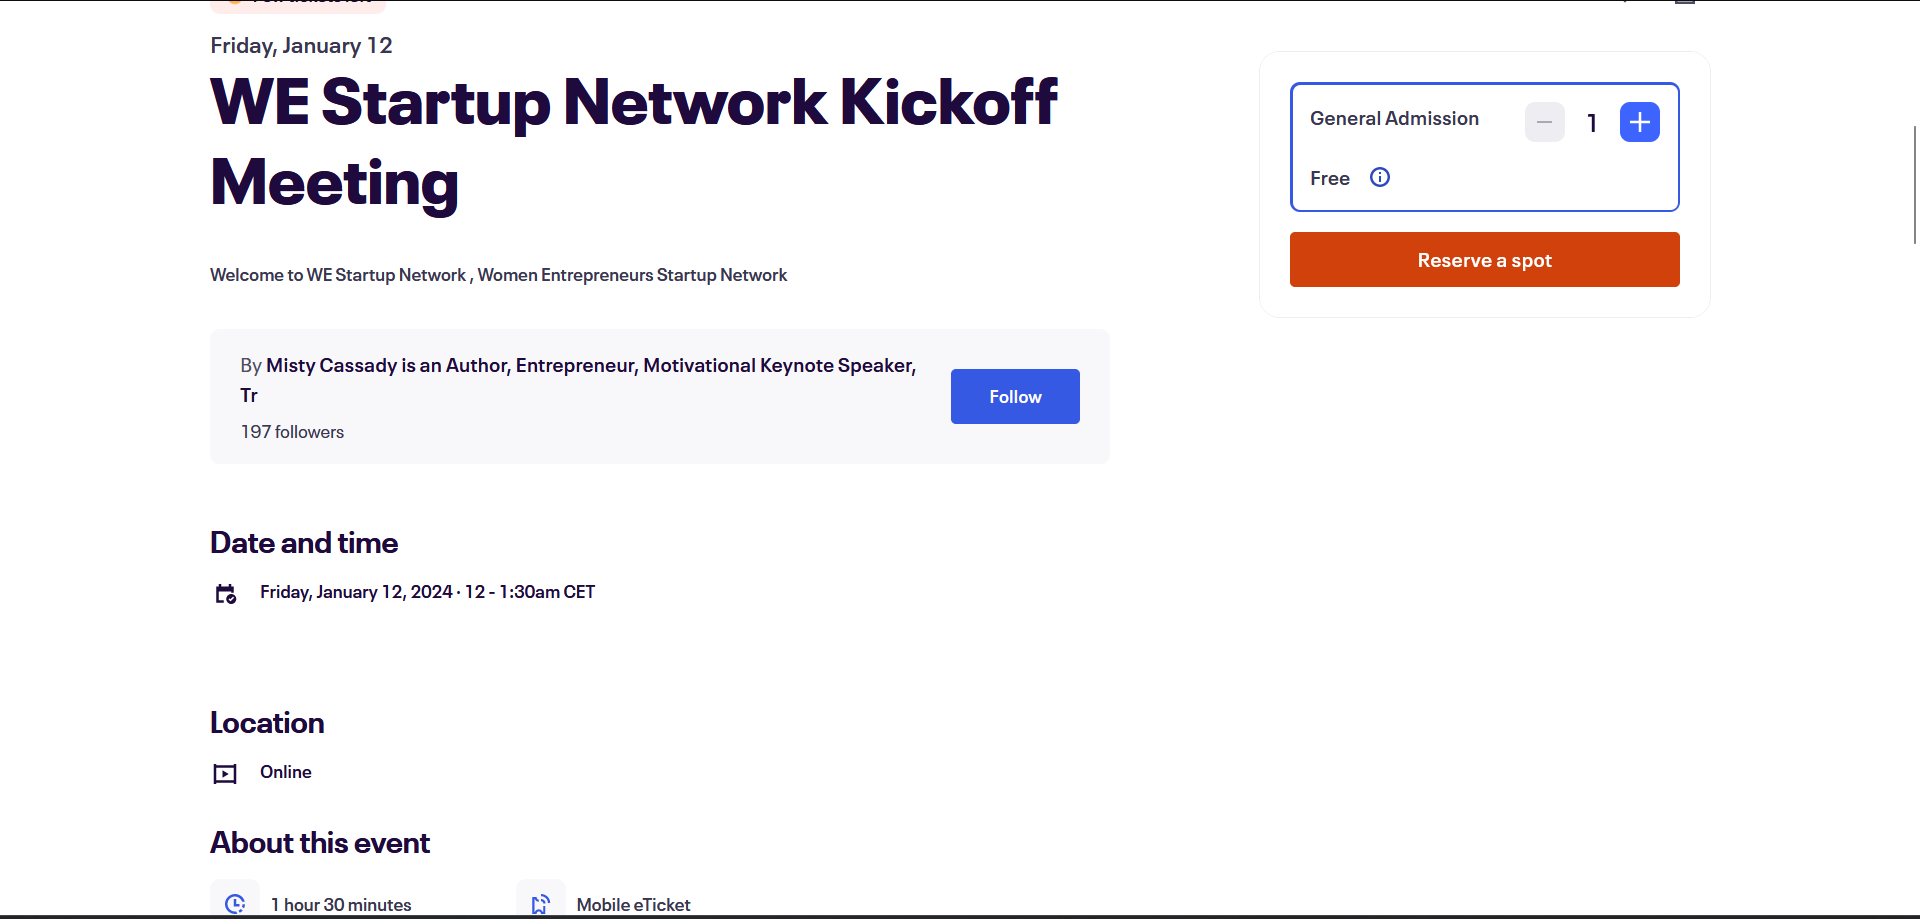
\includegraphics[scale=0.35]{imgs/solutions/eventbrite.png}
    \end{center}
    \caption{Strona przykładowego wydarzenia na platformie Eventbrite}
    \label{rys:ev_interfejs}
    \end{figure}